\documentclass{article}
\usepackage[utf8]{inputenc}

\title{Efficient and Reliable Filesystem Snapshot Distribution}
\author{Lauri Võsandi}
\date{January 2015}

\usepackage{natbib}
\usepackage{graphicx}
\usepackage{url}
\usepackage{tikz}

\begin{document}

\maketitle

\section{Introduction}

TODO

\section{Background}

The foundation of current work was established while author was setting up
the infrastructure to deploy Ubuntu 12.04 LTS on the PC-s of educational
institutions of Tallinn as part of the ongoing efforts of Tallinn Education
Department to switch from proprietary solutions to open-source software.

Puppet was set up to manage Ubuntu workstations remotely. Local IT-support
took the role of bootstrapping the machines and joining them to remote
management server.


\section{Specification}

Customer A runs hundreds of embedded ARM computers for digital signage.
Software is currently updated by mailing the customer an SD-card with
updated software. The customer would prefer to update software and
media over the air but the software update atomicity has to be guaranteed
in order to avoid non-booting machines.

Customer B is about to deploy thousands of Ubuntu netbooks to be used as
remote workstations around the globe. It vital to unroll security updates
as soon as possible, but at the same time it's necessary to guarantee
software update atomicity as the IT helpdesk is lacking in the remote
locations where the machines are used.
The solution has to be installable at customer premises and it
must make use of standard and recognized security methods.

Customer C has around thousand PC-s that need to be converted to Ubuntu,
but the budget is lacking and therefore manual labour has to be minimized.
Glitch-free software update mechanism is crucial part of minimizing manual
labour.

\section{Current approaches}

There are various  currently used to manage Linux based workstations.
In this chapter a background of different methods is outlined.
Subsequently a specification is derived from the needs of customers of
the author. 


\subsection{SaltStack}
TODO

\subsection{Puppet and Foreman}

Puppet is a remote management system which features its own declarative
domain-specific language to describe the state of the configuration
\footnote{http://puppetlabs.com/}. Puppet server also known as Puppetmaster
hosts the configuration while managed machines run puppet agent which polls
the puppetmaster at specified interval, usually 30 minutes. Taken actions
are then reported back to the puppetmaster. Puppet agent and puppetmaster
both are written in Ruby and released the latest versions are released under
liberal Apache 2.0 license. Puppet can be used to manage both Linux and
Windows servers and workstations as well.

Foreman is a complete lifecycle management software for physical and virtual
servers. Foreman incorporates Puppet, a custom web interface and provisioning
tools into single unified application. Even without using provisioning features
Foreman makes one of the most feature-complete web interfaces for Puppet
rivaling the Puppet Dashboard.

\subsection{Chef}

Chef is infrastructure automation tool. Chef is written in Ruby and Erlang. Chef uses domain-specific language written in Ruby.

\subsection{Ansible}

Ansible remote management software uses SSH to connect to the nodes which
means there is no agent running on the managed machine, this however makes
it slightly more complicated to use Ansible no manage machines behind NAT.
Ansible is written in Python and it uses state-driven resource 
written in YAML.

\subsection{Clonezilla}

Clonezilla combines various open-source tools into a single cloning suite.
Clonezilla uses partclone utilities  \footnote{http://partclone.org/} to
identify and transfer only used blocks of various filesystems, most notably
NTFS, ext4 and Btrfs. Clonezilla can be used to grow fielsystems on the fly
making it possible to use same prepared image for disks of various size. 

\subsection{Jails, OpenVZ and LXC}

Jails have been available in FreeBSD since version 4.x. Jails use chroot
syscall to substitute root filesystem of a process making it possible to
create a restricted environment which is isolated from the rest of the
operating system
\footnote{https://www.freebsd.org/doc/en/books/handbook/jails.html}.

The main issue with jails is that dependencies of the target application have
to be available in the jail root filesystem. For instance a Python application
which has modules loaded before chroot operation could operate without any
files in the chroot, but shell script which relies on several executables need
to have those utilities available in chroot as well. With copy-on-write and de
duplicating filesystems the problem how ever becomes irrelevant as root
filesystem of the chroots can be duplicated with no significant overhead.


\subsection{Docker and Rocket}

Docker started off as a way to automate container deployment and configuration
using containers and cgroups present in Linux kernel. As Docker started to add
features that CoreOS developers deemed excessive an alternative project Rocket
was founded
\footnote{\url{http://www.theregister.co.uk/2014/12/03/coreos_rocket_deep_dive/}}.

\subsection{CoreOS and Ubuntu Core}

CoreOS \footnote{https://coreos.com/} is a rearchitected Linux distribution
which provides minimalist foundation to run containers.
It uses two-partition scheme to provide atomic updates of the root filesystem.
The operating system runs off a read-only filesystem while the other one
can be patched runtime. Reboot or \emph{kexec} can be used to boot into
the updated system.
This prevents rendering device unbootable due to interrupted upgrade.

Ubuntu Core is an Ubuntu flavour tailored towards Internet of Things and as a
container platform.
Ubuntu Core introduced root filesystem transactional
updates to Ubuntu using Snappy
\footnote{http://developer.ubuntu.com/en/snappy/}.
Ubuntu Core is designed to run Docker applications and can be used.
Snappy is also plays important role in Ubuntu Phone ecosystem.
Snappy uses OverlayFS (?) to implement transactional updates 


\subsection{OverlayFS}

OverlayFS is a feature introduced in Linux 3.18 which makes it possible to merge contents of two separate mountpoints on the fly.
OpenWrt uses OverlayFS to implement writable JFFS2 layer on top of read-only SquashFS filesystem
\footnote{https://git.kernel.org/cgit/linux/kernel/git/torvalds/linux.git/tree/Documentation/filesystems/overlayfs.txt}.

\subsection{LVM, mdadm and dmraid}

Ext4 has been primary filesystem for Linux based workstations and servers for
a while. It provides filesystem primitives such as files, directories,
permissions and timestamping. In order to add redundancy either software RAID
or logical volume management (LVM) can be used.

Software RAID is implemented in Linux by means of \emph{mdadm}. Software RAID
can be used to build RAID1, RAID0, RAID10/01, RAID5 or RAID6 arrays without
dedicated RAID controller which could also impose a vendor lock-in.

LVM enables pooling of drives, mirroring and snapshotting by adding an
abstraction layer on top of physcal disks. Any filesystem that can be deployed
on physical disk can also be deployed on top of LVM's logical volume. The
kernel takes care of mapping logical addresses to corresponding disk's physical
address. The snapshotting feature of LVM however has been claimed to be buggy
\footnote{http://lwn.net/Articles/522073/}.

\subsection{Btrfs and ZFS}

Btrfs and ZFS both are modern copy on write filesystem for Linux which also
fills in the role of volume manager. Btrfs has been claimed to be unstable but
the situation has improved significantly over the past year or two. 

During snapshot send/receive an optimal parent snapshot is identified and that
is used as basis for the differential snapshot. The Btrfs stream contains
filesystem operations that are indended to be replayed on a clone of the
parent subvolume: create file, \emph{mkdir}, \emph{mknod}, \emph{mkfifo},
symlink, \emph{link}, \emph{unlink}, \emph{rename}, \emph{rmdir}, open file,
close file, write to file, set/remove extended attributes, truncate file,
\emph{chmod}, \emph{chown}
\footnote{http://git.kernel.org/cgit/linux/kernel/git/kdave/btrfs-progs.git/tree/cmds-receive.c}.

Debian has supported Btrfs since Squeeze and has improved support since then
\footnote{https://wiki.debian.org/Btrfs}.  

Facebook has been testing Btrfs in production since the April of 2014
\footnote{\url{https://btrfs.wiki.kernel.org/index.php/Production_Users}}.
Chris Mason, a lead developer of Btrfs joined Facebook in the end of 2013
\footnote{\url{http://article.gmane.org/gmane.comp.file-systems.btrfs/30420}}.
RAID5/6 support and improved data scrubbing for Btrfs was released with Linux
3.19 \footnote{http://lkml.iu.edu/hypermail/linux/kernel/1412.1/03583.html}.


\subsection{FreeNAS, Rockstor and OpenMediaVault}

FreeNAS is a FreeBSD \footnote{http://www.freenas.org/}
based distribution which builds a complete NAS solution on top of
ZFS filesystem and web interface.
Rockstor \footnote{http://rockstor.com/}
is a complementary CentOS based solution that uses Btrfs instead
of ZFS filesystem.
OpenMediaVault provides similar functionality using Debian instead of CentOS
\footnote{http://www.openmediavault.org/}.
All three of them support SMB/CIFS (Windows file shares),
NFS (UNIX file shares) and filesystem aided snapshots.


\subsection{apt-btrfs-snapshot and yum-fs-snapshot}

In Ubuntu package repositories there is available \emph{apt-btrfs-snapshot}
\footnote{https://launchpad.net/apt-btrfs-snapshot} package,
which creates snapshot of the root filesystem before every
\emph{apt-get} operation.

\emph{yum-plugin-fs-snapshot}
\footnote{\url{http://man7.org/linux/man-pages/man1/yum-fs-snapshot.1.html}}
is the corresponding package for Fedora and
Red Hat based distributions.

These approaches make it possible to boot into previous snapshots
in case there are issues with the updated packages.


\subsection{OpenWrt and DD-WRT}

Most Linux based open-source router firmwares originate from Linksys WRT54G
wireless router.
Initially Cisco did not provide source code for the router as GPL mandates.
Between 2003-2008 Free Software Foundation attempted to work with Cisco
to work out issues, but as Cisco continued to release new devices with similar
issues Free Software Foundation eventually sued Cisco for malpractice.
After the lawsuit Cisco complied and has been releasing firmware sources for
all of their devices which make use of software released under GPL licenses.
\footnote{http://www.fsf.org/licensing/2008-12-cisco-complaint}.
Linksys WRT54G sources were basis for various Linux distributions for routers such as
DD-WRT \footnote{http://www.dd-wrt.com/},
Tomato \footnote{http://www.polarcloud.com/tomato}
OpenWrt \footnote{https://openwrt.org/}.

OpenWrt as we know it today is a Linux distribution for embedded devices
which attempts to provide writable filesystem and package management.
OpenWrt supported hardware list mainly targets routers, but other devices are
listed as well \footnote{http://wiki.openwrt.org/toh/}. OpenWrt can be used to
extend lifetime of equipment that otherwise would be largely obsolete due
to unmaintained software from hardware manufacturer.

Most high-end consumer grade routeres employ 8MB NAND Flash chip which is
directly connected to the SoC without controller
\footnote{http://wiki.openwrt.org/doc/techref/flash.layout}.
The Flash storage is usually partitioned at least as 3 slices:
bootloader, read-only root filesystem, read-write overlay.

The read-only root filesystem contains SquashFS
\footnote{http://squashfs.sourceforge.net/}
which is highly-efficient compressed read-only filesystem that support variety
of compression The read-write overlay partition is formatted as JFFS2
(journalling flash filesystem).

This method makes it possible to: perform factory reset simply by formatting
the JFFS2 partition and upgrading firmware by overwriting SquashFS partition.
Due to lack of redundancy in consumer-grade routers an interrupted firmware
upgrade usually renders device unfit for use. This is also known as
\emph{bricking} in embedded developer jargon.


\subsection{Android}

Android ROM images are typically distributed as zip files which contain 
binary blobs for modem and bootloader in addition to snapshots of the
file primary filesystems of Android: boot, cache, recovery, system and userdata
\footnote{https://dl.google.com/dl/android/aosp/shamu-lrx22c-factory-ff173fc6.tgz}.
Differential images are also available, in that case zip file contains
directory tree of files intended to be overwritten or added to the original
root filesystem and post-installation scripts which correct the file permissions
\footnote{http://gapps.itvends.com/gapps-lp-20141212-signed.zip}.

ROM manager such as ClockworkMod \footnote{https://www.clockworkmod.com/} or
TWRP \footnote{http://teamw.in/project/twrp2} has to be used to install or patch
third-party ROM-s.
An alternative Fastboot method is also present in most
Android devices and it can be used to directly write raw filesystem images and
unlock the device
\footnote{\url{http://wiki.cyanogenmod.org/w/Doc:_fastboot_intro}}.




\subsection{OpenStack}

OpenStack is a free and open-source cloud computing software platform
which is composed of several components of which most noteworthy for current work are:
Glance image service, Ironic bare metal provisioning,
Swift object storage and Cinder block storage.
Glance provides discovery, registery and retrieval services of virtual machine images
\footnote{http://docs.openstack.org/developer/glance/}.
Glance BitTorrent delivery enabled BitTorrent support for transferring the images
\footnote{https://blueprints.launchpad.net/glance/+spec/glance-bittorrent-delivery}.


\section{Analysis}

Ubuntu package management fits most scenarios, but there are some rough edges:
package list corruption
\footnote{http://askubuntu.com/questions/532200/14-04-lts-apt-get-segfault},
faulty scripting in packages
\footnote{\url{https://www.linuxquestions.org/questions/showthread.php?s=e0e2f7689f847a56e8cee94a0cafd6bd&p=5216367#post5216367}},
bandwidth overhead etc.

Release upgrades for example from Ubuntu 12.04 to Ubuntu 14.04
have proven to be especially troublesome due to the fact that system libraries
and files are updated and interrupted release upgrade may leave system
in an unusable state.

Debian community has been working hard to provide differential updates for
the packages, but as of February 2015 the efforts have proven fruitless.
Differential updates are applied for package lists
\footnote{\url{https://www.debian-administration.org/article/439/Avoiding_slow_package_updates_with_package_diffs}},
but binary diffs for packages have not implemented yet.
Fedora community has however successfully deployed differential pacakges
\footnote{http://fedoraproject.org/wiki/Features/Presto},
thus reducing the amount of data needed to be transferred during an pacakge update. For bigger software (eg LibreOffice) the lack of differential updates poses a serious concern, especially for low-bandwidth links.

Puppet, SaltStack, Chef, Ansible and other traditional configuration management
fit best the scenario where each node has slightly different configuration and
it makes sense to keep them separate. However provisioning very similar nodes
with for instance Foreman has obvious overhead - each node has to fetch updated
packages independently from the same APT repositories, same has to be done for
application software.

\section{Prototype}

Using Debian, Ubuntu and Gentoo were evaluated as provisioning utility
operating system. With Debian and Ubuntu the resulting PXE bootable image
would have exceeded 100MB.
As of February of 2015 the CoreOS image suffers similar issue -
\emph{vmlinuz}
\footnote{\url{http://stable.release.core-os.net/amd64-usr/current/coreos_production_pxe.vmlinuz}}
and
\emph{initrd}
\footnote{\url{http://stable.release.core-os.net/amd64-usr/current/coreos_production_pxe_image.cpio.gz}}
files required to boot over PXE are correspondingly 24MB and 117MB.
With Gentoo significant tweaking is required, because Gentoo is
mainly targeted for power users.

Using Python to build pseudo-graphic menu-driven user interface was
evaluated and deemed not necessary for the goal as Python runtime and
dependant libraries add about 10MB to the resulting image.
In addition to that \emph{parted} Python bindings were unavailable
in Buildroot package selection.

Buildroot was eventually used to generate an compact 10MB all-in-one
PXE-bootable image. Utilities \emph{dialog} in conjunction with
\emph{curl}, \emph{jq} and others were used to build the user-interface
and Bash was used to program the user-interface logic.
The security model for the initial deployment phase could be improved
as only method of verification of the source is the certificate
authority chain verified by \emph{curl} during the Btrfs snapshot
retrieval.

LXC containers are used to bootstrap the template for provisioning.
With Btrfs backing store on top of a Btrfs filesystem the container
can be saved in an isolated Btrfs subvolume which makes it easy to
snapshot the container.
Within the container \emph{puppet apply} and similar methods can be used
to take advantage of already existing configuration management know-how.
Otherwise traditional manual labour can be employed to set up the template.
During the release phase the LXC container is stopped, pre-release scripts
are executed to clean up package cache and temporary files.
Then a read-only Btrfs snapshot is generated from the container root filesystem.
At this point new snapshot becomes available for other nodes.

For running nodes a DBus service was written to poll the snapshot server
for updates and another DBus service was written in Python to notify user
about available updates.

\begin{figure}[!htb]
\centering
\scalebox{0.5}{% Graphic for TeX using PGF
% Title: /home/lauri/Projektid/blog/pages/cloning/dia/workflow-en.dia
% Creator: Dia v0.97.2
% CreationDate: Thu Feb 26 18:06:28 2015
% For: lauri
% \usepackage{tikz}
% The following commands are not supported in PSTricks at present
% We define them conditionally, so when they are implemented,
% this pgf file will use them.
\ifx\du\undefined
  \newlength{\du}
\fi
\setlength{\du}{15\unitlength}
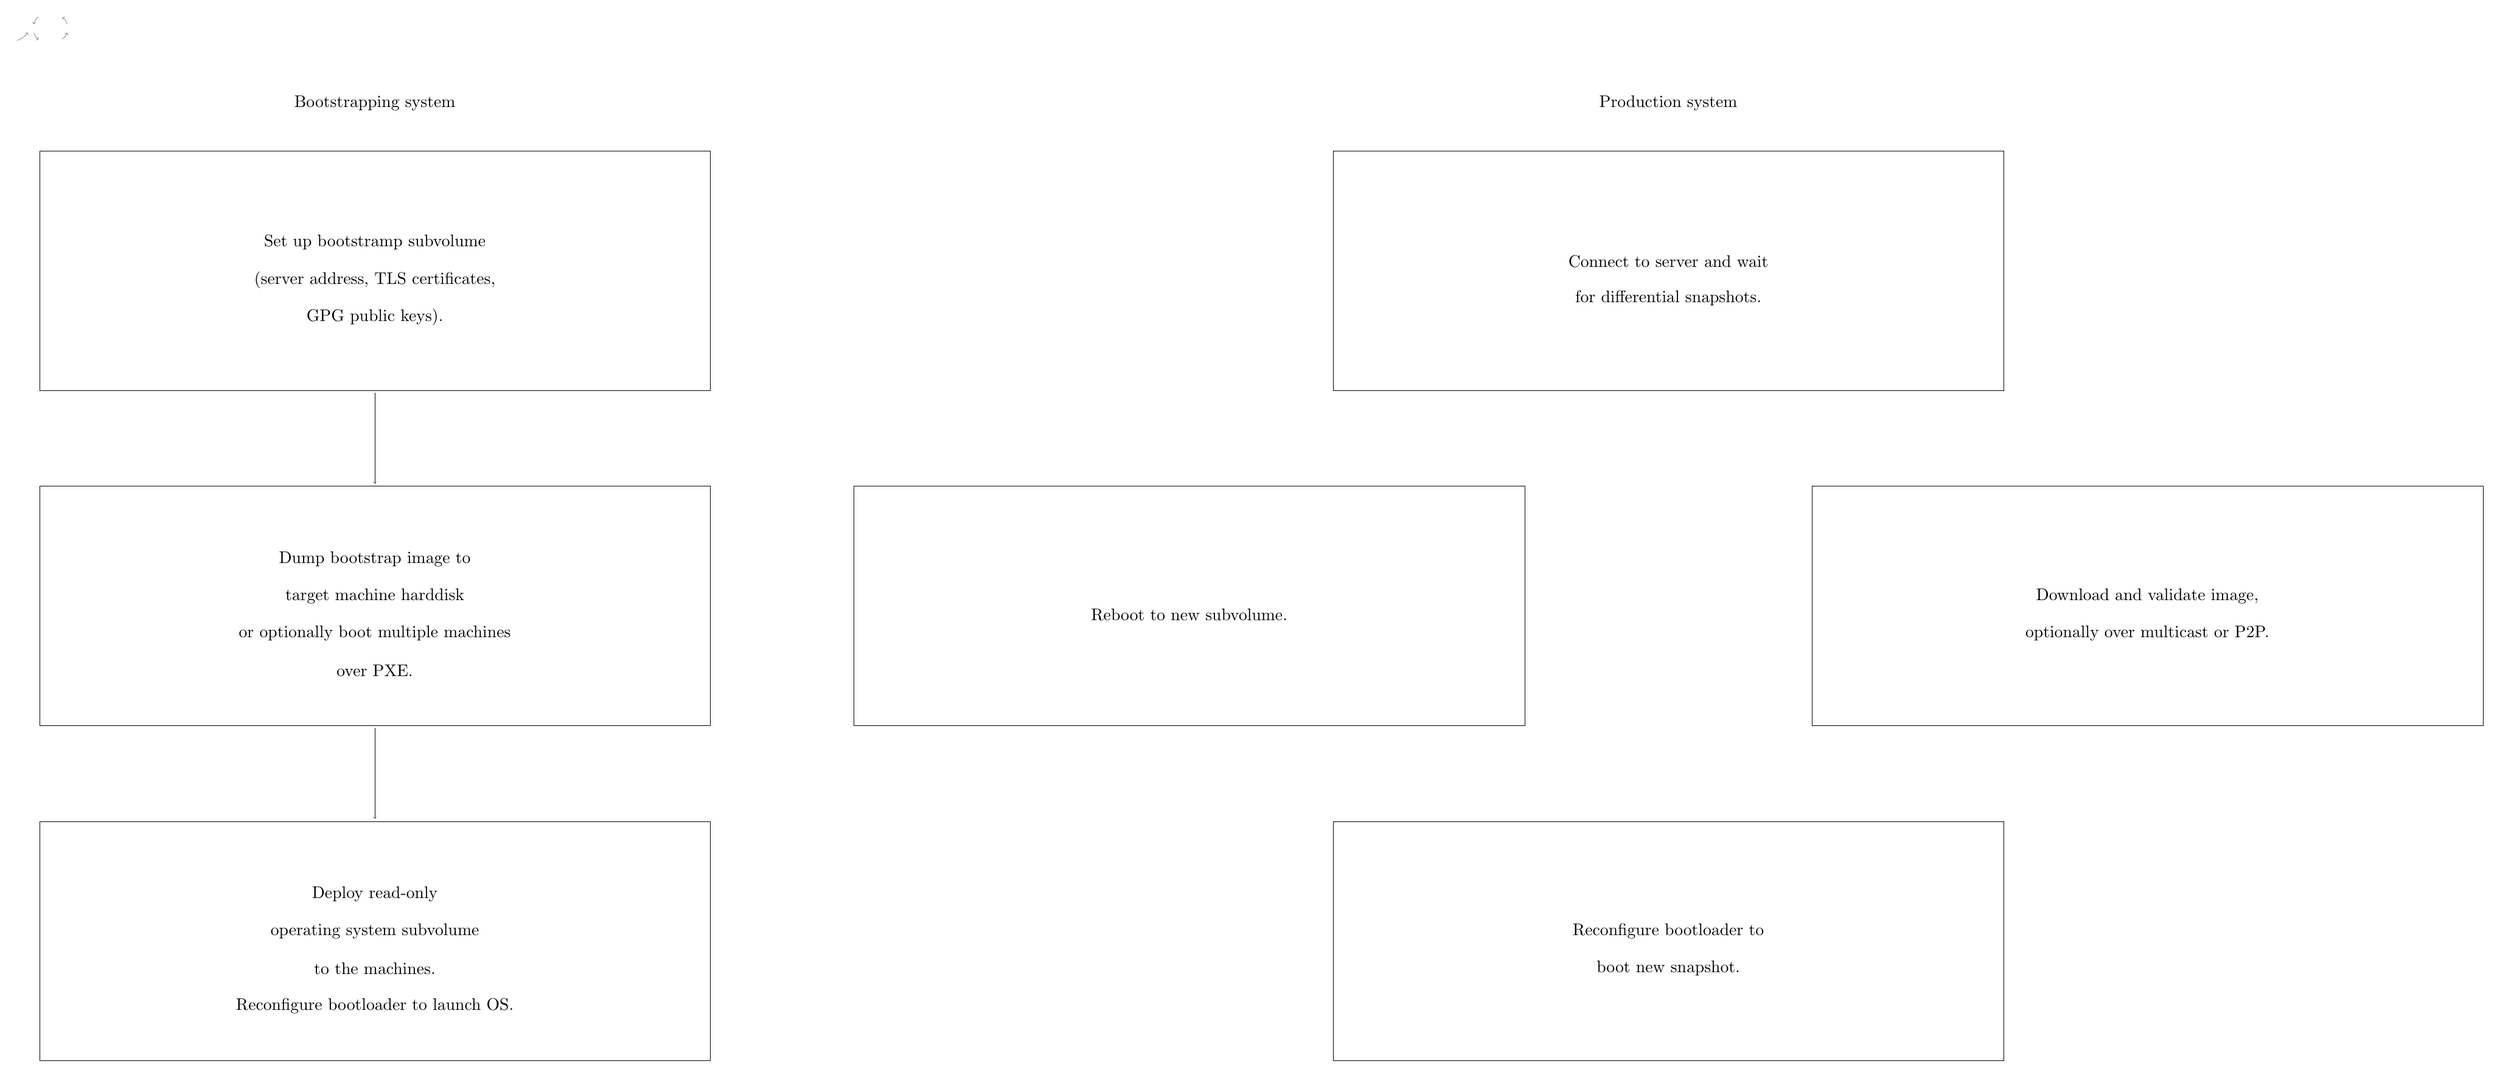
\begin{tikzpicture}
\pgftransformxscale{1.000000}
\pgftransformyscale{-1.000000}
\definecolor{dialinecolor}{rgb}{0.000000, 0.000000, 0.000000}
\pgfsetstrokecolor{dialinecolor}
\definecolor{dialinecolor}{rgb}{1.000000, 1.000000, 1.000000}
\pgfsetfillcolor{dialinecolor}
% setfont left to latex
\definecolor{dialinecolor}{rgb}{0.000000, 0.000000, 0.000000}
\pgfsetstrokecolor{dialinecolor}
\node at (8.000000\du,2.000000\du){Bootstrapping system};
\definecolor{dialinecolor}{rgb}{1.000000, 1.000000, 1.000000}
\pgfsetfillcolor{dialinecolor}
\fill (1.000000\du,3.000000\du)--(1.000000\du,8.000000\du)--(15.000000\du,8.000000\du)--(15.000000\du,3.000000\du)--cycle;
\pgfsetlinewidth{0.100000\du}
\pgfsetdash{}{0pt}
\pgfsetdash{}{0pt}
\pgfsetmiterjoin
\definecolor{dialinecolor}{rgb}{0.000000, 0.000000, 0.000000}
\pgfsetstrokecolor{dialinecolor}
\draw (1.000000\du,3.000000\du)--(1.000000\du,8.000000\du)--(15.000000\du,8.000000\du)--(15.000000\du,3.000000\du)--cycle;
% setfont left to latex
\definecolor{dialinecolor}{rgb}{0.000000, 0.000000, 0.000000}
\pgfsetstrokecolor{dialinecolor}
\node at (8.000000\du,4.913333\du){Set up bootstramp subvolume};
% setfont left to latex
\definecolor{dialinecolor}{rgb}{0.000000, 0.000000, 0.000000}
\pgfsetstrokecolor{dialinecolor}
\node at (8.000000\du,5.689444\du){(server address, TLS certificates,};
% setfont left to latex
\definecolor{dialinecolor}{rgb}{0.000000, 0.000000, 0.000000}
\pgfsetstrokecolor{dialinecolor}
\node at (8.000000\du,6.465556\du){GPG public keys).};
\definecolor{dialinecolor}{rgb}{1.000000, 1.000000, 1.000000}
\pgfsetfillcolor{dialinecolor}
\fill (1.000000\du,10.000000\du)--(1.000000\du,15.000000\du)--(15.000000\du,15.000000\du)--(15.000000\du,10.000000\du)--cycle;
\pgfsetlinewidth{0.100000\du}
\pgfsetdash{}{0pt}
\pgfsetdash{}{0pt}
\pgfsetmiterjoin
\definecolor{dialinecolor}{rgb}{0.000000, 0.000000, 0.000000}
\pgfsetstrokecolor{dialinecolor}
\draw (1.000000\du,10.000000\du)--(1.000000\du,15.000000\du)--(15.000000\du,15.000000\du)--(15.000000\du,10.000000\du)--cycle;
% setfont left to latex
\definecolor{dialinecolor}{rgb}{0.000000, 0.000000, 0.000000}
\pgfsetstrokecolor{dialinecolor}
\node at (8.000000\du,11.525278\du){Dump bootstrap image to};
% setfont left to latex
\definecolor{dialinecolor}{rgb}{0.000000, 0.000000, 0.000000}
\pgfsetstrokecolor{dialinecolor}
\node at (8.000000\du,12.301389\du){target machine harddisk};
% setfont left to latex
\definecolor{dialinecolor}{rgb}{0.000000, 0.000000, 0.000000}
\pgfsetstrokecolor{dialinecolor}
\node at (8.000000\du,13.077500\du){or optionally boot multiple machines};
% setfont left to latex
\definecolor{dialinecolor}{rgb}{0.000000, 0.000000, 0.000000}
\pgfsetstrokecolor{dialinecolor}
\node at (8.000000\du,13.853611\du){over PXE.};
\pgfsetlinewidth{0.100000\du}
\pgfsetdash{}{0pt}
\pgfsetdash{}{0pt}
\pgfsetbuttcap
{
\definecolor{dialinecolor}{rgb}{0.000000, 0.000000, 0.000000}
\pgfsetfillcolor{dialinecolor}
% was here!!!
\pgfsetarrowsend{to}
\definecolor{dialinecolor}{rgb}{0.000000, 0.000000, 0.000000}
\pgfsetstrokecolor{dialinecolor}
\draw (8.000000\du,8.050232\du)--(8.000000\du,9.949768\du);
}
\definecolor{dialinecolor}{rgb}{1.000000, 1.000000, 1.000000}
\pgfsetfillcolor{dialinecolor}
\fill (1.000000\du,17.000000\du)--(1.000000\du,22.000000\du)--(15.000000\du,22.000000\du)--(15.000000\du,17.000000\du)--cycle;
\pgfsetlinewidth{0.100000\du}
\pgfsetdash{}{0pt}
\pgfsetdash{}{0pt}
\pgfsetmiterjoin
\definecolor{dialinecolor}{rgb}{0.000000, 0.000000, 0.000000}
\pgfsetstrokecolor{dialinecolor}
\draw (1.000000\du,17.000000\du)--(1.000000\du,22.000000\du)--(15.000000\du,22.000000\du)--(15.000000\du,17.000000\du)--cycle;
% setfont left to latex
\definecolor{dialinecolor}{rgb}{0.000000, 0.000000, 0.000000}
\pgfsetstrokecolor{dialinecolor}
\node at (8.000000\du,18.525278\du){Deploy read-only};
% setfont left to latex
\definecolor{dialinecolor}{rgb}{0.000000, 0.000000, 0.000000}
\pgfsetstrokecolor{dialinecolor}
\node at (8.000000\du,19.301389\du){operating system subvolume};
% setfont left to latex
\definecolor{dialinecolor}{rgb}{0.000000, 0.000000, 0.000000}
\pgfsetstrokecolor{dialinecolor}
\node at (8.000000\du,20.077500\du){to the machines.};
% setfont left to latex
\definecolor{dialinecolor}{rgb}{0.000000, 0.000000, 0.000000}
\pgfsetstrokecolor{dialinecolor}
\node at (8.000000\du,20.853611\du){Reconfigure bootloader to launch OS.};
\pgfsetlinewidth{0.100000\du}
\pgfsetdash{}{0pt}
\pgfsetdash{}{0pt}
\pgfsetbuttcap
{
\definecolor{dialinecolor}{rgb}{0.000000, 0.000000, 0.000000}
\pgfsetfillcolor{dialinecolor}
% was here!!!
\pgfsetarrowsend{to}
\definecolor{dialinecolor}{rgb}{0.000000, 0.000000, 0.000000}
\pgfsetstrokecolor{dialinecolor}
\draw (8.000000\du,15.050232\du)--(8.000000\du,16.949768\du);
}
\definecolor{dialinecolor}{rgb}{1.000000, 1.000000, 1.000000}
\pgfsetfillcolor{dialinecolor}
\fill (28.000000\du,3.000000\du)--(28.000000\du,8.000000\du)--(42.000000\du,8.000000\du)--(42.000000\du,3.000000\du)--cycle;
\pgfsetlinewidth{0.100000\du}
\pgfsetdash{}{0pt}
\pgfsetdash{}{0pt}
\pgfsetmiterjoin
\definecolor{dialinecolor}{rgb}{0.000000, 0.000000, 0.000000}
\pgfsetstrokecolor{dialinecolor}
\draw (28.000000\du,3.000000\du)--(28.000000\du,8.000000\du)--(42.000000\du,8.000000\du)--(42.000000\du,3.000000\du)--cycle;
% setfont left to latex
\definecolor{dialinecolor}{rgb}{0.000000, 0.000000, 0.000000}
\pgfsetstrokecolor{dialinecolor}
\node at (35.000000\du,5.301389\du){Connect to server and wait};
% setfont left to latex
\definecolor{dialinecolor}{rgb}{0.000000, 0.000000, 0.000000}
\pgfsetstrokecolor{dialinecolor}
\node at (35.000000\du,6.077500\du){for differential snapshots.};
\definecolor{dialinecolor}{rgb}{1.000000, 1.000000, 1.000000}
\pgfsetfillcolor{dialinecolor}
\fill (18.000000\du,10.000000\du)--(18.000000\du,15.000000\du)--(32.000000\du,15.000000\du)--(32.000000\du,10.000000\du)--cycle;
\pgfsetlinewidth{0.100000\du}
\pgfsetdash{}{0pt}
\pgfsetdash{}{0pt}
\pgfsetmiterjoin
\definecolor{dialinecolor}{rgb}{0.000000, 0.000000, 0.000000}
\pgfsetstrokecolor{dialinecolor}
\draw (18.000000\du,10.000000\du)--(18.000000\du,15.000000\du)--(32.000000\du,15.000000\du)--(32.000000\du,10.000000\du)--cycle;
% setfont left to latex
\definecolor{dialinecolor}{rgb}{0.000000, 0.000000, 0.000000}
\pgfsetstrokecolor{dialinecolor}
\node at (25.000000\du,12.689444\du){Reboot to new subvolume.};
\pgfsetlinewidth{0.100000\du}
\pgfsetdash{}{0pt}
\pgfsetdash{}{0pt}
\pgfsetbuttcap
{
\definecolor{dialinecolor}{rgb}{0.000000, 0.000000, 0.000000}
\pgfsetfillcolor{dialinecolor}
% was here!!!
\pgfsetarrowsend{to}
\definecolor{dialinecolor}{rgb}{0.000000, 0.000000, 0.000000}
\pgfsetstrokecolor{dialinecolor}
\pgfpathmoveto{\pgfpoint{15.049490\du}{19.640275\du}}
\pgfpatharc{74}{35}{11.858541\du and 11.858541\du}
\pgfusepath{stroke}
}
\definecolor{dialinecolor}{rgb}{1.000000, 1.000000, 1.000000}
\pgfsetfillcolor{dialinecolor}
\fill (28.000000\du,17.000000\du)--(28.000000\du,22.000000\du)--(42.000000\du,22.000000\du)--(42.000000\du,17.000000\du)--cycle;
\pgfsetlinewidth{0.100000\du}
\pgfsetdash{}{0pt}
\pgfsetdash{}{0pt}
\pgfsetmiterjoin
\definecolor{dialinecolor}{rgb}{0.000000, 0.000000, 0.000000}
\pgfsetstrokecolor{dialinecolor}
\draw (28.000000\du,17.000000\du)--(28.000000\du,22.000000\du)--(42.000000\du,22.000000\du)--(42.000000\du,17.000000\du)--cycle;
% setfont left to latex
\definecolor{dialinecolor}{rgb}{0.000000, 0.000000, 0.000000}
\pgfsetstrokecolor{dialinecolor}
\node at (35.000000\du,19.301389\du){Reconfigure bootloader to};
% setfont left to latex
\definecolor{dialinecolor}{rgb}{0.000000, 0.000000, 0.000000}
\pgfsetstrokecolor{dialinecolor}
\node at (35.000000\du,20.077500\du){boot new snapshot.};
\definecolor{dialinecolor}{rgb}{1.000000, 1.000000, 1.000000}
\pgfsetfillcolor{dialinecolor}
\fill (38.000000\du,10.000000\du)--(38.000000\du,15.000000\du)--(52.000000\du,15.000000\du)--(52.000000\du,10.000000\du)--cycle;
\pgfsetlinewidth{0.100000\du}
\pgfsetdash{}{0pt}
\pgfsetdash{}{0pt}
\pgfsetmiterjoin
\definecolor{dialinecolor}{rgb}{0.000000, 0.000000, 0.000000}
\pgfsetstrokecolor{dialinecolor}
\draw (38.000000\du,10.000000\du)--(38.000000\du,15.000000\du)--(52.000000\du,15.000000\du)--(52.000000\du,10.000000\du)--cycle;
% setfont left to latex
\definecolor{dialinecolor}{rgb}{0.000000, 0.000000, 0.000000}
\pgfsetstrokecolor{dialinecolor}
\node at (45.000000\du,12.301389\du){Download and validate image,};
% setfont left to latex
\definecolor{dialinecolor}{rgb}{0.000000, 0.000000, 0.000000}
\pgfsetstrokecolor{dialinecolor}
\node at (45.000000\du,13.077500\du){optionally over multicast or P2P.};
\pgfsetlinewidth{0.100000\du}
\pgfsetdash{}{0pt}
\pgfsetdash{}{0pt}
\pgfsetbuttcap
{
\definecolor{dialinecolor}{rgb}{0.000000, 0.000000, 0.000000}
\pgfsetfillcolor{dialinecolor}
% was here!!!
\pgfsetarrowsend{to}
\definecolor{dialinecolor}{rgb}{0.000000, 0.000000, 0.000000}
\pgfsetstrokecolor{dialinecolor}
\pgfpathmoveto{\pgfpoint{27.950110\du}{5.675501\du}}
\pgfpatharc{237}{192}{6.723537\du and 6.723537\du}
\pgfusepath{stroke}
}
\pgfsetlinewidth{0.100000\du}
\pgfsetdash{}{0pt}
\pgfsetdash{}{0pt}
\pgfsetbuttcap
{
\definecolor{dialinecolor}{rgb}{0.000000, 0.000000, 0.000000}
\pgfsetfillcolor{dialinecolor}
% was here!!!
\pgfsetarrowsend{to}
\definecolor{dialinecolor}{rgb}{0.000000, 0.000000, 0.000000}
\pgfsetstrokecolor{dialinecolor}
\pgfpathmoveto{\pgfpoint{44.870667\du}{9.950218\du}}
\pgfpatharc{347}{305}{6.860399\du and 6.860399\du}
\pgfusepath{stroke}
}
\pgfsetlinewidth{0.100000\du}
\pgfsetdash{}{0pt}
\pgfsetdash{}{0pt}
\pgfsetbuttcap
{
\definecolor{dialinecolor}{rgb}{0.000000, 0.000000, 0.000000}
\pgfsetfillcolor{dialinecolor}
% was here!!!
\pgfsetarrowsend{to}
\definecolor{dialinecolor}{rgb}{0.000000, 0.000000, 0.000000}
\pgfsetstrokecolor{dialinecolor}
\pgfpathmoveto{\pgfpoint{42.049045\du}{18.901522\du}}
\pgfpatharc{55}{16}{7.019442\du and 7.019442\du}
\pgfusepath{stroke}
}
\pgfsetlinewidth{0.100000\du}
\pgfsetdash{}{0pt}
\pgfsetdash{}{0pt}
\pgfsetbuttcap
{
\definecolor{dialinecolor}{rgb}{0.000000, 0.000000, 0.000000}
\pgfsetfillcolor{dialinecolor}
% was here!!!
\pgfsetarrowsend{to}
\definecolor{dialinecolor}{rgb}{0.000000, 0.000000, 0.000000}
\pgfsetstrokecolor{dialinecolor}
\pgfpathmoveto{\pgfpoint{25.129248\du}{15.049431\du}}
\pgfpatharc{167}{125}{6.860399\du and 6.860399\du}
\pgfusepath{stroke}
}
% setfont left to latex
\definecolor{dialinecolor}{rgb}{0.000000, 0.000000, 0.000000}
\pgfsetstrokecolor{dialinecolor}
\node at (35.000000\du,2.000000\du){Production system};
\end{tikzpicture}
}
\caption{Workflow for btrfs snapshot based software deployment}
\label{fig:digraph}
\end{figure}

\begin{figure}[!htb]
\centering
\scalebox{0.5}{% Graphic for TeX using PGF
% Title: /home/lauri/msc-thesis/dia/traditional-partitioning.dia
% Creator: Dia v0.97.3
% CreationDate: Sun Apr  5 10:02:27 2015
% For: lauri
% \usepackage{tikz}
% The following commands are not supported in PSTricks at present
% We define them conditionally, so when they are implemented,
% this pgf file will use them.
\ifx\du\undefined
  \newlength{\du}
\fi
\setlength{\du}{15\unitlength}
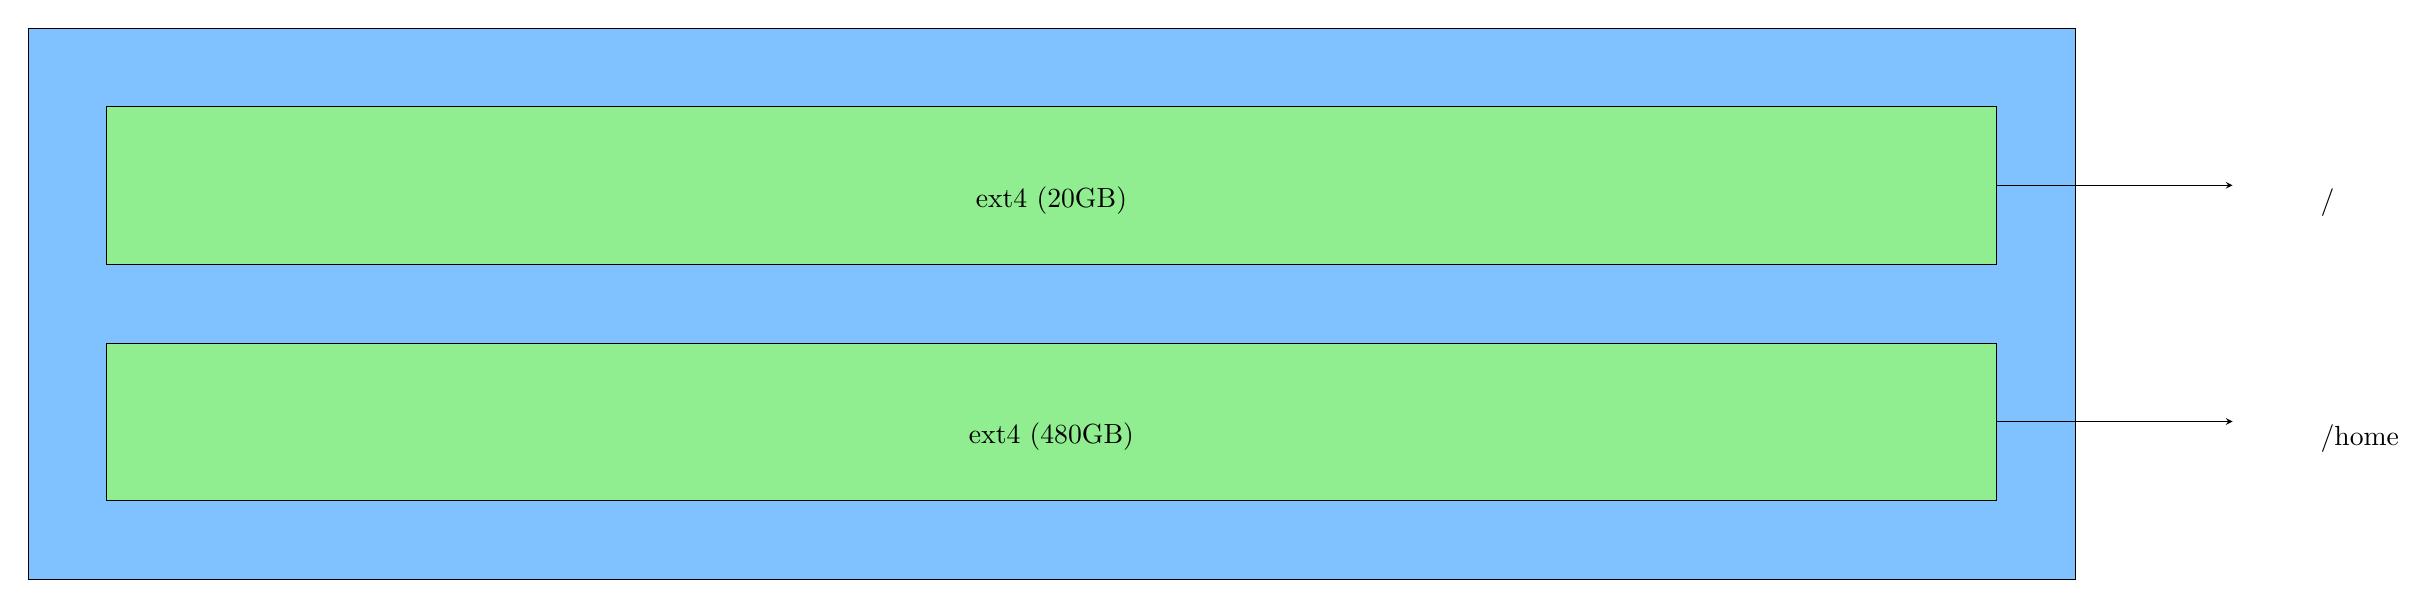
\begin{tikzpicture}
\pgftransformxscale{1.000000}
\pgftransformyscale{-1.000000}
\definecolor{dialinecolor}{rgb}{0.000000, 0.000000, 0.000000}
\pgfsetstrokecolor{dialinecolor}
\definecolor{dialinecolor}{rgb}{1.000000, 1.000000, 1.000000}
\pgfsetfillcolor{dialinecolor}
\pgfsetlinewidth{0.100000\du}
\pgfsetdash{}{0pt}
\pgfsetdash{}{0pt}
\pgfsetmiterjoin
\definecolor{dialinecolor}{rgb}{0.501961, 0.756863, 1.000000}
\pgfsetfillcolor{dialinecolor}
\fill (0.000000\du,0.000000\du)--(0.000000\du,7.000000\du)--(26.000000\du,7.000000\du)--(26.000000\du,0.000000\du)--cycle;
\definecolor{dialinecolor}{rgb}{0.000000, 0.000000, 0.000000}
\pgfsetstrokecolor{dialinecolor}
\draw (0.000000\du,0.000000\du)--(0.000000\du,7.000000\du)--(26.000000\du,7.000000\du)--(26.000000\du,0.000000\du)--cycle;
\definecolor{dialinecolor}{rgb}{0.564706, 0.933333, 0.564706}
\pgfsetfillcolor{dialinecolor}
\fill (1.000000\du,1.000000\du)--(1.000000\du,3.000000\du)--(25.000000\du,3.000000\du)--(25.000000\du,1.000000\du)--cycle;
\pgfsetlinewidth{0.100000\du}
\pgfsetdash{}{0pt}
\pgfsetdash{}{0pt}
\pgfsetmiterjoin
\definecolor{dialinecolor}{rgb}{0.000000, 0.000000, 0.000000}
\pgfsetstrokecolor{dialinecolor}
\draw (1.000000\du,1.000000\du)--(1.000000\du,3.000000\du)--(25.000000\du,3.000000\du)--(25.000000\du,1.000000\du)--cycle;
% setfont left to latex
\definecolor{dialinecolor}{rgb}{0.000000, 0.000000, 0.000000}
\pgfsetstrokecolor{dialinecolor}
\node at (13.000000\du,2.195000\du){ext4 (20GB)};
\pgfsetlinewidth{0.100000\du}
\pgfsetdash{}{0pt}
\pgfsetdash{}{0pt}
\pgfsetbuttcap
{
\definecolor{dialinecolor}{rgb}{0.000000, 0.000000, 0.000000}
\pgfsetfillcolor{dialinecolor}
% was here!!!
\pgfsetarrowsend{stealth}
\definecolor{dialinecolor}{rgb}{0.000000, 0.000000, 0.000000}
\pgfsetstrokecolor{dialinecolor}
\draw (25.000000\du,2.000000\du)--(28.000000\du,2.000000\du);
}
\pgfsetlinewidth{0.100000\du}
\pgfsetdash{}{0pt}
\pgfsetdash{}{0pt}
\pgfsetbuttcap
{
\definecolor{dialinecolor}{rgb}{0.000000, 0.000000, 0.000000}
\pgfsetfillcolor{dialinecolor}
% was here!!!
\pgfsetarrowsend{stealth}
\definecolor{dialinecolor}{rgb}{0.000000, 0.000000, 0.000000}
\pgfsetstrokecolor{dialinecolor}
\draw (25.000000\du,5.000000\du)--(28.000000\du,5.000000\du);
}
% setfont left to latex
\definecolor{dialinecolor}{rgb}{0.000000, 0.000000, 0.000000}
\pgfsetstrokecolor{dialinecolor}
\node[anchor=west] at (29.000000\du,5.221250\du){/home};
% setfont left to latex
\definecolor{dialinecolor}{rgb}{0.000000, 0.000000, 0.000000}
\pgfsetstrokecolor{dialinecolor}
\node[anchor=west] at (29.000000\du,2.221250\du){/};
\definecolor{dialinecolor}{rgb}{0.564706, 0.933333, 0.564706}
\pgfsetfillcolor{dialinecolor}
\fill (1.000000\du,4.000000\du)--(1.000000\du,6.000000\du)--(25.000000\du,6.000000\du)--(25.000000\du,4.000000\du)--cycle;
\pgfsetlinewidth{0.100000\du}
\pgfsetdash{}{0pt}
\pgfsetdash{}{0pt}
\pgfsetmiterjoin
\definecolor{dialinecolor}{rgb}{0.000000, 0.000000, 0.000000}
\pgfsetstrokecolor{dialinecolor}
\draw (1.000000\du,4.000000\du)--(1.000000\du,6.000000\du)--(25.000000\du,6.000000\du)--(25.000000\du,4.000000\du)--cycle;
% setfont left to latex
\definecolor{dialinecolor}{rgb}{0.000000, 0.000000, 0.000000}
\pgfsetstrokecolor{dialinecolor}
\node at (13.000000\du,5.195000\du){ext4 (480GB)};
\end{tikzpicture}
}
\caption{Traditional partitioning}
\label{fig:digraph}
\end{figure}

\begin{figure}[!htb]
\centering
\scalebox{0.5}{% Graphic for TeX using PGF
% Title: /home/lauri/Projektid/msc-thesis/dia/pooled-partitioning.dia
% Creator: Dia v0.97.2
% CreationDate: Fri May 22 01:33:44 2015
% For: lauri
% \usepackage{tikz}
% The following commands are not supported in PSTricks at present
% We define them conditionally, so when they are implemented,
% this pgf file will use them.
\ifx\du\undefined
  \newlength{\du}
\fi
\setlength{\du}{15\unitlength}
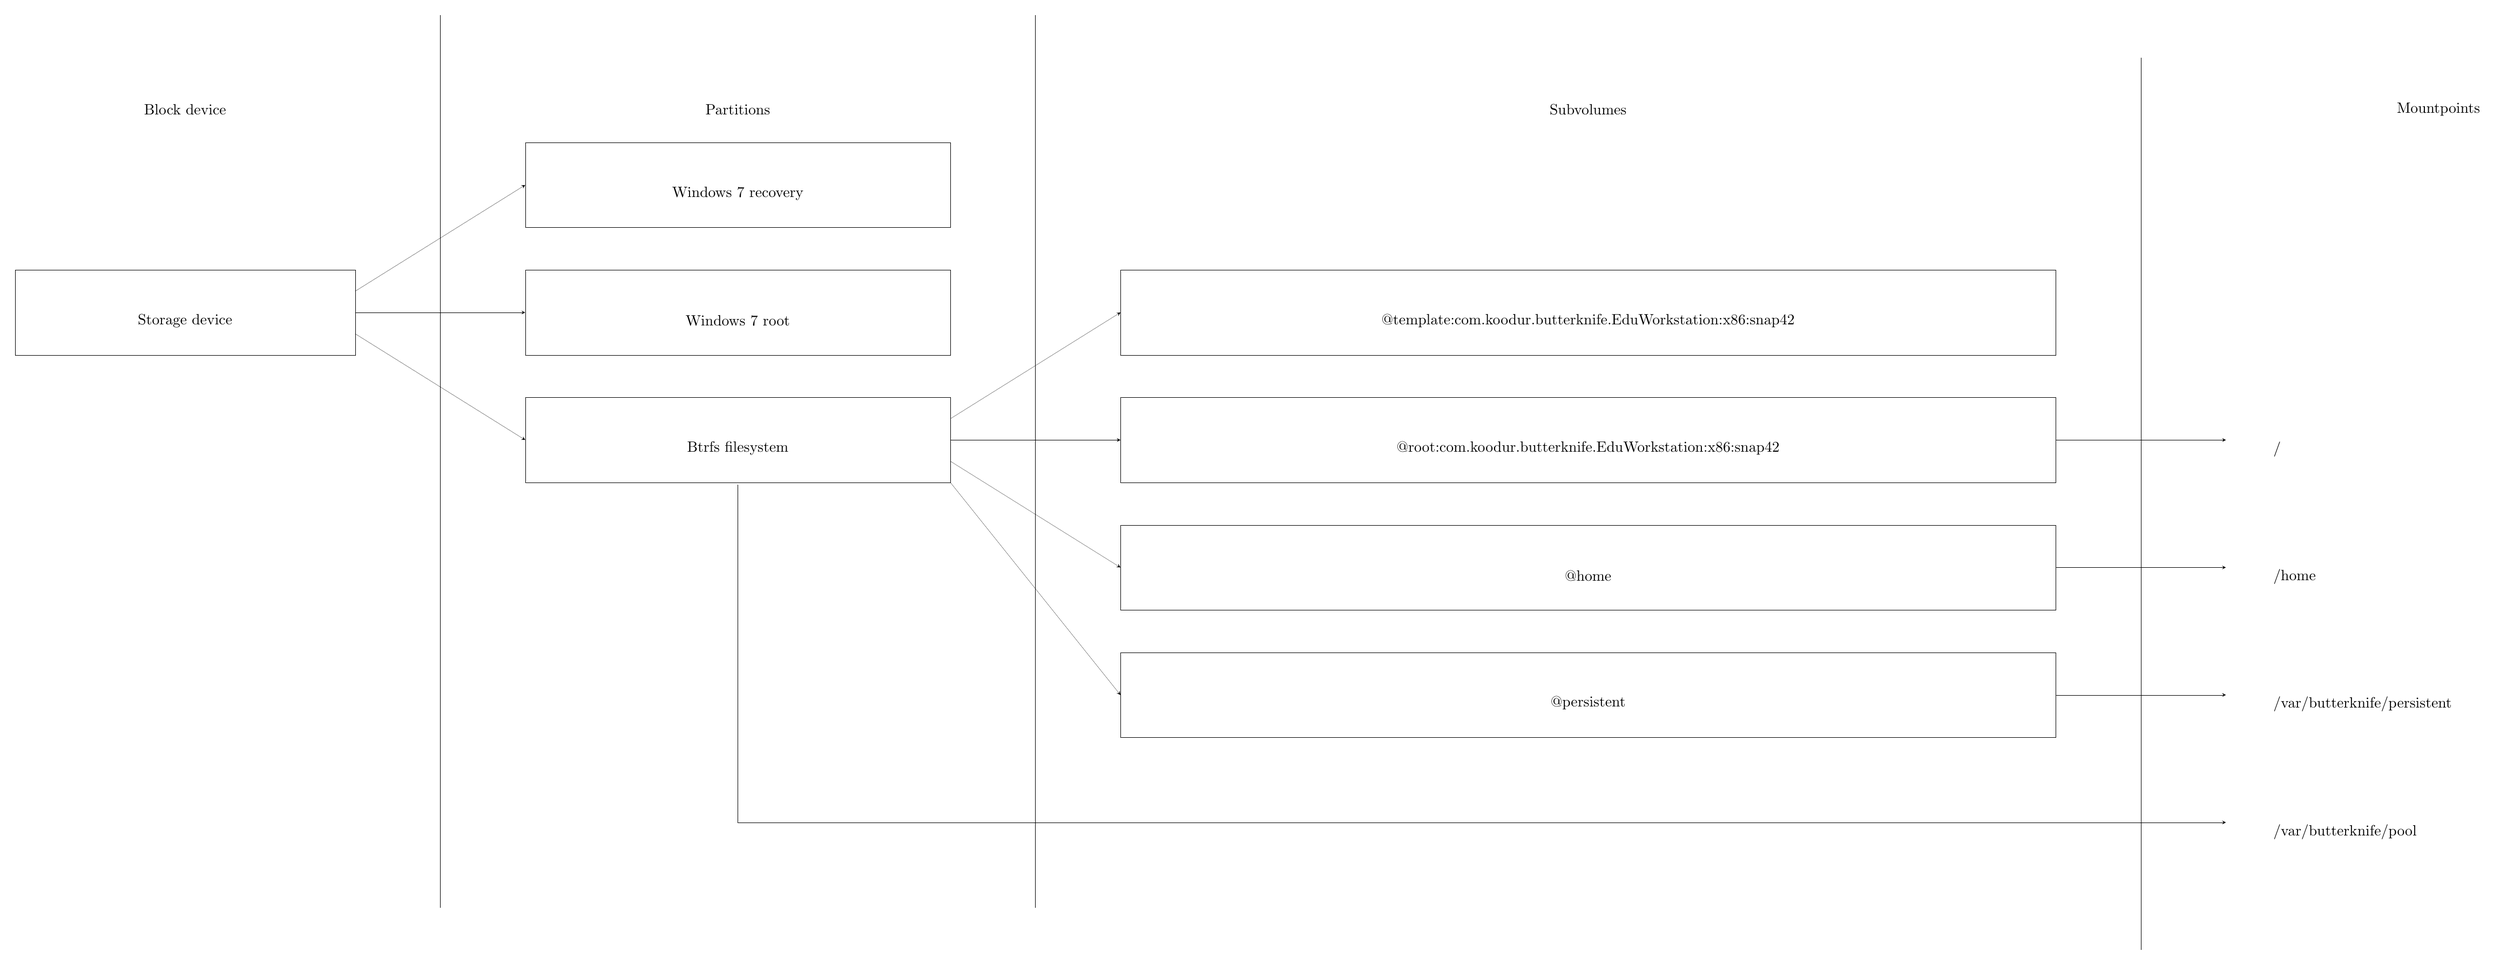
\begin{tikzpicture}
\pgftransformxscale{1.000000}
\pgftransformyscale{-1.000000}
\definecolor{dialinecolor}{rgb}{0.000000, 0.000000, 0.000000}
\pgfsetstrokecolor{dialinecolor}
\definecolor{dialinecolor}{rgb}{1.000000, 1.000000, 1.000000}
\pgfsetfillcolor{dialinecolor}
\definecolor{dialinecolor}{rgb}{1.000000, 1.000000, 1.000000}
\pgfsetfillcolor{dialinecolor}
\fill (27.000000\du,7.000000\du)--(27.000000\du,9.000000\du)--(49.000000\du,9.000000\du)--(49.000000\du,7.000000\du)--cycle;
\pgfsetlinewidth{0.100000\du}
\pgfsetdash{}{0pt}
\pgfsetdash{}{0pt}
\pgfsetmiterjoin
\definecolor{dialinecolor}{rgb}{0.000000, 0.000000, 0.000000}
\pgfsetstrokecolor{dialinecolor}
\draw (27.000000\du,7.000000\du)--(27.000000\du,9.000000\du)--(49.000000\du,9.000000\du)--(49.000000\du,7.000000\du)--cycle;
% setfont left to latex
\definecolor{dialinecolor}{rgb}{0.000000, 0.000000, 0.000000}
\pgfsetstrokecolor{dialinecolor}
\node at (38.000000\du,8.195000\du){@template:com.koodur.butterknife.EduWorkstation:x86:snap42};
\definecolor{dialinecolor}{rgb}{1.000000, 1.000000, 1.000000}
\pgfsetfillcolor{dialinecolor}
\fill (27.000000\du,10.000000\du)--(27.000000\du,12.000000\du)--(49.000000\du,12.000000\du)--(49.000000\du,10.000000\du)--cycle;
\pgfsetlinewidth{0.100000\du}
\pgfsetdash{}{0pt}
\pgfsetdash{}{0pt}
\pgfsetmiterjoin
\definecolor{dialinecolor}{rgb}{0.000000, 0.000000, 0.000000}
\pgfsetstrokecolor{dialinecolor}
\draw (27.000000\du,10.000000\du)--(27.000000\du,12.000000\du)--(49.000000\du,12.000000\du)--(49.000000\du,10.000000\du)--cycle;
% setfont left to latex
\definecolor{dialinecolor}{rgb}{0.000000, 0.000000, 0.000000}
\pgfsetstrokecolor{dialinecolor}
\node at (38.000000\du,11.195000\du){@root:com.koodur.butterknife.EduWorkstation:x86:snap42};
\definecolor{dialinecolor}{rgb}{1.000000, 1.000000, 1.000000}
\pgfsetfillcolor{dialinecolor}
\fill (27.000000\du,13.000000\du)--(27.000000\du,15.000000\du)--(49.000000\du,15.000000\du)--(49.000000\du,13.000000\du)--cycle;
\pgfsetlinewidth{0.100000\du}
\pgfsetdash{}{0pt}
\pgfsetdash{}{0pt}
\pgfsetmiterjoin
\definecolor{dialinecolor}{rgb}{0.000000, 0.000000, 0.000000}
\pgfsetstrokecolor{dialinecolor}
\draw (27.000000\du,13.000000\du)--(27.000000\du,15.000000\du)--(49.000000\du,15.000000\du)--(49.000000\du,13.000000\du)--cycle;
% setfont left to latex
\definecolor{dialinecolor}{rgb}{0.000000, 0.000000, 0.000000}
\pgfsetstrokecolor{dialinecolor}
\node at (38.000000\du,14.195000\du){@home};
\definecolor{dialinecolor}{rgb}{1.000000, 1.000000, 1.000000}
\pgfsetfillcolor{dialinecolor}
\fill (27.000000\du,16.000000\du)--(27.000000\du,18.000000\du)--(49.000000\du,18.000000\du)--(49.000000\du,16.000000\du)--cycle;
\pgfsetlinewidth{0.100000\du}
\pgfsetdash{}{0pt}
\pgfsetdash{}{0pt}
\pgfsetmiterjoin
\definecolor{dialinecolor}{rgb}{0.000000, 0.000000, 0.000000}
\pgfsetstrokecolor{dialinecolor}
\draw (27.000000\du,16.000000\du)--(27.000000\du,18.000000\du)--(49.000000\du,18.000000\du)--(49.000000\du,16.000000\du)--cycle;
% setfont left to latex
\definecolor{dialinecolor}{rgb}{0.000000, 0.000000, 0.000000}
\pgfsetstrokecolor{dialinecolor}
\node at (38.000000\du,17.195000\du){@persistent};
\pgfsetlinewidth{0.100000\du}
\pgfsetdash{}{0pt}
\pgfsetdash{}{0pt}
\pgfsetbuttcap
{
\definecolor{dialinecolor}{rgb}{0.000000, 0.000000, 0.000000}
\pgfsetfillcolor{dialinecolor}
% was here!!!
\pgfsetarrowsend{stealth}
\definecolor{dialinecolor}{rgb}{0.000000, 0.000000, 0.000000}
\pgfsetstrokecolor{dialinecolor}
\draw (49.000000\du,11.000000\du)--(53.000000\du,11.000000\du);
}
\pgfsetlinewidth{0.100000\du}
\pgfsetdash{}{0pt}
\pgfsetdash{}{0pt}
\pgfsetbuttcap
{
\definecolor{dialinecolor}{rgb}{0.000000, 0.000000, 0.000000}
\pgfsetfillcolor{dialinecolor}
% was here!!!
\pgfsetarrowsend{stealth}
\definecolor{dialinecolor}{rgb}{0.000000, 0.000000, 0.000000}
\pgfsetstrokecolor{dialinecolor}
\draw (49.000000\du,14.000000\du)--(53.000000\du,14.000000\du);
}
\pgfsetlinewidth{0.100000\du}
\pgfsetdash{}{0pt}
\pgfsetdash{}{0pt}
\pgfsetbuttcap
{
\definecolor{dialinecolor}{rgb}{0.000000, 0.000000, 0.000000}
\pgfsetfillcolor{dialinecolor}
% was here!!!
\pgfsetarrowsend{stealth}
\definecolor{dialinecolor}{rgb}{0.000000, 0.000000, 0.000000}
\pgfsetstrokecolor{dialinecolor}
\draw (49.000000\du,17.000000\du)--(53.000000\du,17.000000\du);
}
% setfont left to latex
\definecolor{dialinecolor}{rgb}{0.000000, 0.000000, 0.000000}
\pgfsetstrokecolor{dialinecolor}
\node[anchor=west] at (54.000000\du,14.221250\du){/home};
% setfont left to latex
\definecolor{dialinecolor}{rgb}{0.000000, 0.000000, 0.000000}
\pgfsetstrokecolor{dialinecolor}
\node[anchor=west] at (54.000000\du,17.221250\du){/var/butterknife/persistent};
% setfont left to latex
\definecolor{dialinecolor}{rgb}{0.000000, 0.000000, 0.000000}
\pgfsetstrokecolor{dialinecolor}
\node[anchor=west] at (54.000000\du,11.221250\du){/};
% setfont left to latex
\definecolor{dialinecolor}{rgb}{0.000000, 0.000000, 0.000000}
\pgfsetstrokecolor{dialinecolor}
\node[anchor=west] at (54.000000\du,20.221250\du){/var/butterknife/pool};
\definecolor{dialinecolor}{rgb}{1.000000, 1.000000, 1.000000}
\pgfsetfillcolor{dialinecolor}
\fill (1.000000\du,7.000000\du)--(1.000000\du,9.000000\du)--(9.000000\du,9.000000\du)--(9.000000\du,7.000000\du)--cycle;
\pgfsetlinewidth{0.100000\du}
\pgfsetdash{}{0pt}
\pgfsetdash{}{0pt}
\pgfsetmiterjoin
\definecolor{dialinecolor}{rgb}{0.000000, 0.000000, 0.000000}
\pgfsetstrokecolor{dialinecolor}
\draw (1.000000\du,7.000000\du)--(1.000000\du,9.000000\du)--(9.000000\du,9.000000\du)--(9.000000\du,7.000000\du)--cycle;
% setfont left to latex
\definecolor{dialinecolor}{rgb}{0.000000, 0.000000, 0.000000}
\pgfsetstrokecolor{dialinecolor}
\node at (5.000000\du,8.195000\du){Storage device};
\definecolor{dialinecolor}{rgb}{1.000000, 1.000000, 1.000000}
\pgfsetfillcolor{dialinecolor}
\fill (13.000000\du,4.000000\du)--(13.000000\du,6.000000\du)--(23.000000\du,6.000000\du)--(23.000000\du,4.000000\du)--cycle;
\pgfsetlinewidth{0.100000\du}
\pgfsetdash{}{0pt}
\pgfsetdash{}{0pt}
\pgfsetmiterjoin
\definecolor{dialinecolor}{rgb}{0.000000, 0.000000, 0.000000}
\pgfsetstrokecolor{dialinecolor}
\draw (13.000000\du,4.000000\du)--(13.000000\du,6.000000\du)--(23.000000\du,6.000000\du)--(23.000000\du,4.000000\du)--cycle;
% setfont left to latex
\definecolor{dialinecolor}{rgb}{0.000000, 0.000000, 0.000000}
\pgfsetstrokecolor{dialinecolor}
\node at (18.000000\du,5.195000\du){Windows 7 recovery};
\definecolor{dialinecolor}{rgb}{1.000000, 1.000000, 1.000000}
\pgfsetfillcolor{dialinecolor}
\fill (13.000000\du,10.000000\du)--(13.000000\du,12.000000\du)--(23.000000\du,12.000000\du)--(23.000000\du,10.000000\du)--cycle;
\pgfsetlinewidth{0.100000\du}
\pgfsetdash{}{0pt}
\pgfsetdash{}{0pt}
\pgfsetmiterjoin
\definecolor{dialinecolor}{rgb}{0.000000, 0.000000, 0.000000}
\pgfsetstrokecolor{dialinecolor}
\draw (13.000000\du,10.000000\du)--(13.000000\du,12.000000\du)--(23.000000\du,12.000000\du)--(23.000000\du,10.000000\du)--cycle;
% setfont left to latex
\definecolor{dialinecolor}{rgb}{0.000000, 0.000000, 0.000000}
\pgfsetstrokecolor{dialinecolor}
\node at (18.000000\du,11.195000\du){Btrfs filesystem};
\definecolor{dialinecolor}{rgb}{1.000000, 1.000000, 1.000000}
\pgfsetfillcolor{dialinecolor}
\fill (13.000000\du,7.000000\du)--(13.000000\du,9.000000\du)--(23.000000\du,9.000000\du)--(23.000000\du,7.000000\du)--cycle;
\pgfsetlinewidth{0.100000\du}
\pgfsetdash{}{0pt}
\pgfsetdash{}{0pt}
\pgfsetmiterjoin
\definecolor{dialinecolor}{rgb}{0.000000, 0.000000, 0.000000}
\pgfsetstrokecolor{dialinecolor}
\draw (13.000000\du,7.000000\du)--(13.000000\du,9.000000\du)--(23.000000\du,9.000000\du)--(23.000000\du,7.000000\du)--cycle;
% setfont left to latex
\definecolor{dialinecolor}{rgb}{0.000000, 0.000000, 0.000000}
\pgfsetstrokecolor{dialinecolor}
\node at (18.000000\du,8.195000\du){Windows 7 root};
\pgfsetlinewidth{0.100000\du}
\pgfsetdash{}{0pt}
\pgfsetdash{}{0pt}
\pgfsetbuttcap
{
\definecolor{dialinecolor}{rgb}{0.000000, 0.000000, 0.000000}
\pgfsetfillcolor{dialinecolor}
% was here!!!
\pgfsetarrowsend{stealth}
\definecolor{dialinecolor}{rgb}{0.000000, 0.000000, 0.000000}
\pgfsetstrokecolor{dialinecolor}
\draw (23.000000\du,10.500000\du)--(27.000000\du,8.000000\du);
}
\pgfsetlinewidth{0.100000\du}
\pgfsetdash{}{0pt}
\pgfsetdash{}{0pt}
\pgfsetbuttcap
{
\definecolor{dialinecolor}{rgb}{0.000000, 0.000000, 0.000000}
\pgfsetfillcolor{dialinecolor}
% was here!!!
\pgfsetarrowsend{stealth}
\definecolor{dialinecolor}{rgb}{0.000000, 0.000000, 0.000000}
\pgfsetstrokecolor{dialinecolor}
\draw (23.000000\du,11.000000\du)--(27.000000\du,11.000000\du);
}
\pgfsetlinewidth{0.100000\du}
\pgfsetdash{}{0pt}
\pgfsetdash{}{0pt}
\pgfsetbuttcap
{
\definecolor{dialinecolor}{rgb}{0.000000, 0.000000, 0.000000}
\pgfsetfillcolor{dialinecolor}
% was here!!!
\pgfsetarrowsend{stealth}
\definecolor{dialinecolor}{rgb}{0.000000, 0.000000, 0.000000}
\pgfsetstrokecolor{dialinecolor}
\draw (23.000000\du,11.500000\du)--(27.000000\du,14.000000\du);
}
\pgfsetlinewidth{0.100000\du}
\pgfsetdash{}{0pt}
\pgfsetdash{}{0pt}
\pgfsetbuttcap
{
\definecolor{dialinecolor}{rgb}{0.000000, 0.000000, 0.000000}
\pgfsetfillcolor{dialinecolor}
% was here!!!
\pgfsetarrowsend{stealth}
\definecolor{dialinecolor}{rgb}{0.000000, 0.000000, 0.000000}
\pgfsetstrokecolor{dialinecolor}
\draw (9.000000\du,7.500000\du)--(13.000000\du,5.000000\du);
}
\pgfsetlinewidth{0.100000\du}
\pgfsetdash{}{0pt}
\pgfsetdash{}{0pt}
\pgfsetbuttcap
{
\definecolor{dialinecolor}{rgb}{0.000000, 0.000000, 0.000000}
\pgfsetfillcolor{dialinecolor}
% was here!!!
\pgfsetarrowsend{stealth}
\definecolor{dialinecolor}{rgb}{0.000000, 0.000000, 0.000000}
\pgfsetstrokecolor{dialinecolor}
\draw (9.000000\du,8.000000\du)--(13.000000\du,8.000000\du);
}
\pgfsetlinewidth{0.100000\du}
\pgfsetdash{}{0pt}
\pgfsetdash{}{0pt}
\pgfsetbuttcap
{
\definecolor{dialinecolor}{rgb}{0.000000, 0.000000, 0.000000}
\pgfsetfillcolor{dialinecolor}
% was here!!!
\pgfsetarrowsend{stealth}
\definecolor{dialinecolor}{rgb}{0.000000, 0.000000, 0.000000}
\pgfsetstrokecolor{dialinecolor}
\draw (9.000000\du,8.500000\du)--(13.000000\du,11.000000\du);
}
\pgfsetlinewidth{0.100000\du}
\pgfsetdash{}{0pt}
\pgfsetdash{}{0pt}
\pgfsetbuttcap
{
\definecolor{dialinecolor}{rgb}{0.000000, 0.000000, 0.000000}
\pgfsetfillcolor{dialinecolor}
% was here!!!
\pgfsetarrowsend{stealth}
\definecolor{dialinecolor}{rgb}{0.000000, 0.000000, 0.000000}
\pgfsetstrokecolor{dialinecolor}
\draw (23.000000\du,12.000000\du)--(27.000000\du,17.000000\du);
}
% setfont left to latex
\definecolor{dialinecolor}{rgb}{0.000000, 0.000000, 0.000000}
\pgfsetstrokecolor{dialinecolor}
\node at (5.000000\du,3.221250\du){Block device};
% setfont left to latex
\definecolor{dialinecolor}{rgb}{0.000000, 0.000000, 0.000000}
\pgfsetstrokecolor{dialinecolor}
\node at (18.000000\du,3.221250\du){Partitions};
% setfont left to latex
\definecolor{dialinecolor}{rgb}{0.000000, 0.000000, 0.000000}
\pgfsetstrokecolor{dialinecolor}
\node at (38.000000\du,3.221250\du){Subvolumes};
\pgfsetlinewidth{0.100000\du}
\pgfsetdash{{\pgflinewidth}{0.200000\du}}{0cm}
\pgfsetdash{{\pgflinewidth}{0.200000\du}}{0cm}
\pgfsetbuttcap
{
\definecolor{dialinecolor}{rgb}{0.000000, 0.000000, 0.000000}
\pgfsetfillcolor{dialinecolor}
% was here!!!
\definecolor{dialinecolor}{rgb}{0.000000, 0.000000, 0.000000}
\pgfsetstrokecolor{dialinecolor}
\draw (11.000000\du,1.000000\du)--(11.000000\du,22.000000\du);
}
\pgfsetlinewidth{0.100000\du}
\pgfsetdash{{\pgflinewidth}{0.200000\du}}{0cm}
\pgfsetdash{{\pgflinewidth}{0.200000\du}}{0cm}
\pgfsetbuttcap
{
\definecolor{dialinecolor}{rgb}{0.000000, 0.000000, 0.000000}
\pgfsetfillcolor{dialinecolor}
% was here!!!
\definecolor{dialinecolor}{rgb}{0.000000, 0.000000, 0.000000}
\pgfsetstrokecolor{dialinecolor}
\draw (25.000000\du,1.000000\du)--(25.000000\du,22.000000\du);
}
\pgfsetlinewidth{0.100000\du}
\pgfsetdash{{\pgflinewidth}{0.200000\du}}{0cm}
\pgfsetdash{{\pgflinewidth}{0.200000\du}}{0cm}
\pgfsetbuttcap
{
\definecolor{dialinecolor}{rgb}{0.000000, 0.000000, 0.000000}
\pgfsetfillcolor{dialinecolor}
% was here!!!
\definecolor{dialinecolor}{rgb}{0.000000, 0.000000, 0.000000}
\pgfsetstrokecolor{dialinecolor}
\draw (51.000000\du,2.000000\du)--(51.000000\du,23.000000\du);
}
% setfont left to latex
\definecolor{dialinecolor}{rgb}{0.000000, 0.000000, 0.000000}
\pgfsetstrokecolor{dialinecolor}
\node at (58.000000\du,3.221250\du){Mountpoints};
\pgfsetlinewidth{0.100000\du}
\pgfsetdash{}{0pt}
\pgfsetdash{}{0pt}
\pgfsetmiterjoin
\pgfsetbuttcap
{
\definecolor{dialinecolor}{rgb}{0.000000, 0.000000, 0.000000}
\pgfsetfillcolor{dialinecolor}
% was here!!!
\pgfsetarrowsend{stealth}
{\pgfsetcornersarced{\pgfpoint{0.000000\du}{0.000000\du}}\definecolor{dialinecolor}{rgb}{0.000000, 0.000000, 0.000000}
\pgfsetstrokecolor{dialinecolor}
\draw (18.000000\du,12.048096\du)--(18.000000\du,20.000000\du)--(53.000000\du,20.000000\du);
}}
\end{tikzpicture}
}
\caption{Pooled partitioning}
\label{fig:digraph}
\end{figure}


\section{Conclusion}

TODO


\section{Future work}

\subsection{Btrfs and BitTorrent integration}

Btrfs uses crc32c for checksumming and support for alternative checksum algorithms is planned.
Current on-disk format supports up to 256-bit hash checksum per
metadata block and arbitrary count of blocks for per-block checksums.
\footnote{\url{https://btrfs.wiki.kernel.org/index.php/FAQ#What_checksum_function_does_Btrfs_use.3F}}
As of November 2013 Btrfs defaults to 16KB or page size whichever
is larger.
On most Linux workstation page size is set to 4KB, thus 16KB block
size takes precedence.
\footnote{\url{https://git.kernel.org/cgit/linux/kernel/git/mason/btrfs-progs.git/commit/?id=c652e4efb8e2dd76ef1627d8cd649c6af5905902}}

BitTorrent splits files into pieces and SHA-1 hash is calculated per piece.
BitTorrent protocol does not specify minimal piece length
\footnote{\url{http://www.bittorrent.org/beps/bep_0003.html#info-dictionary}},
but for example libtorrent imposes restriction of having piece length
a multiple of 16KB
\footnote{\url{http://www.libtorrent.org/reference-Create_Torrents.html#id5}}.

As online deduplication is in works for Btrfs it makes sense to combine the two,
implementing additional \emph{ioctl} for Btrfs in order to perform block lookup
by checksum is trivial task.
This could make it possible to implement high-performance BitTorrent seedbox
which takes advantage of Btrfs metadata.

\subsection{Alternative filesystem layouts}

Lennart Poettering, an controversial Free Software developer has outlined a method
\footnote{http://0pointer.net/blog/revisiting-how-we-put-together-linux-systems.html}
of building Linux based systems using Btrfs snapshots.
The new layout requires significant effort from operating system distributors,
software suite vendors but promises significant save of effort on testing
software on Linux based systems.

Debian has put significant effort into making Debian package builds reproducible
\footnote{https://wiki.debian.org/ReproducibleBuilds}.



\bibliographystyle{plain}
\bibliography{references}

\end{document}
